\section{Тест производительности}

Убедимся, что построенный жадный алгоритм действительно имеет линейную сложность. Для этого замерим время работы программы на нескольких тестах: с последовательностями длин 100, 1000, 10000, 100000, 1000000, 10000000.

\begin{alltt}
roma@DESKTOP-JD58QU2:~/Diskran/lab8$ ./a.out < test1e2
39
Time: 0.000198 s
roma@DESKTOP-JD58QU2:~/Diskran/lab8$ ./a.out < test1e3
350
Time: 0.0002908 s
roma@DESKTOP-JD58QU2:~/Diskran/lab8$ ./a.out < test1e4
3345
Time: 0.0011082 s
roma@DESKTOP-JD58QU2:~/Diskran/lab8$ ./a.out < test1e5
33434
Time: 0.0094662 s
roma@DESKTOP-JD58QU2:~/Diskran/lab8$ ./a.out < test1e6
333194
Time: 0.0914062 s
roma@DESKTOP-JD58QU2:~/Diskran/lab8$ ./a.out < test1e7
3331149
Time: 0.915165 s
\end{alltt}

Отметим полученные результаты на графике.

\begin{center}
	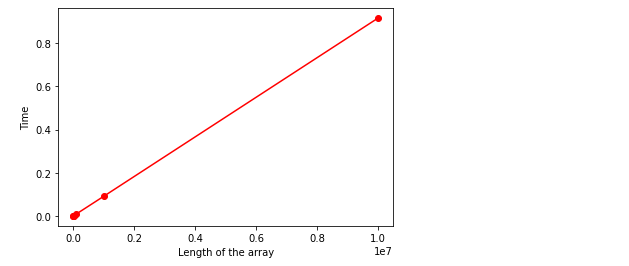
\includegraphics{src/123.png}
\end{center}

По графику видно, что время работы программы возрастает прямо пропорционально объему входных данных, значит сложность программы действительно равна $O(n)$.

\pagebreak

